\pdfoutput=1

\documentclass{standalone}
\usepackage{tikz}
\usetikzlibrary{shapes,arrows,positioning}

\begin{document}

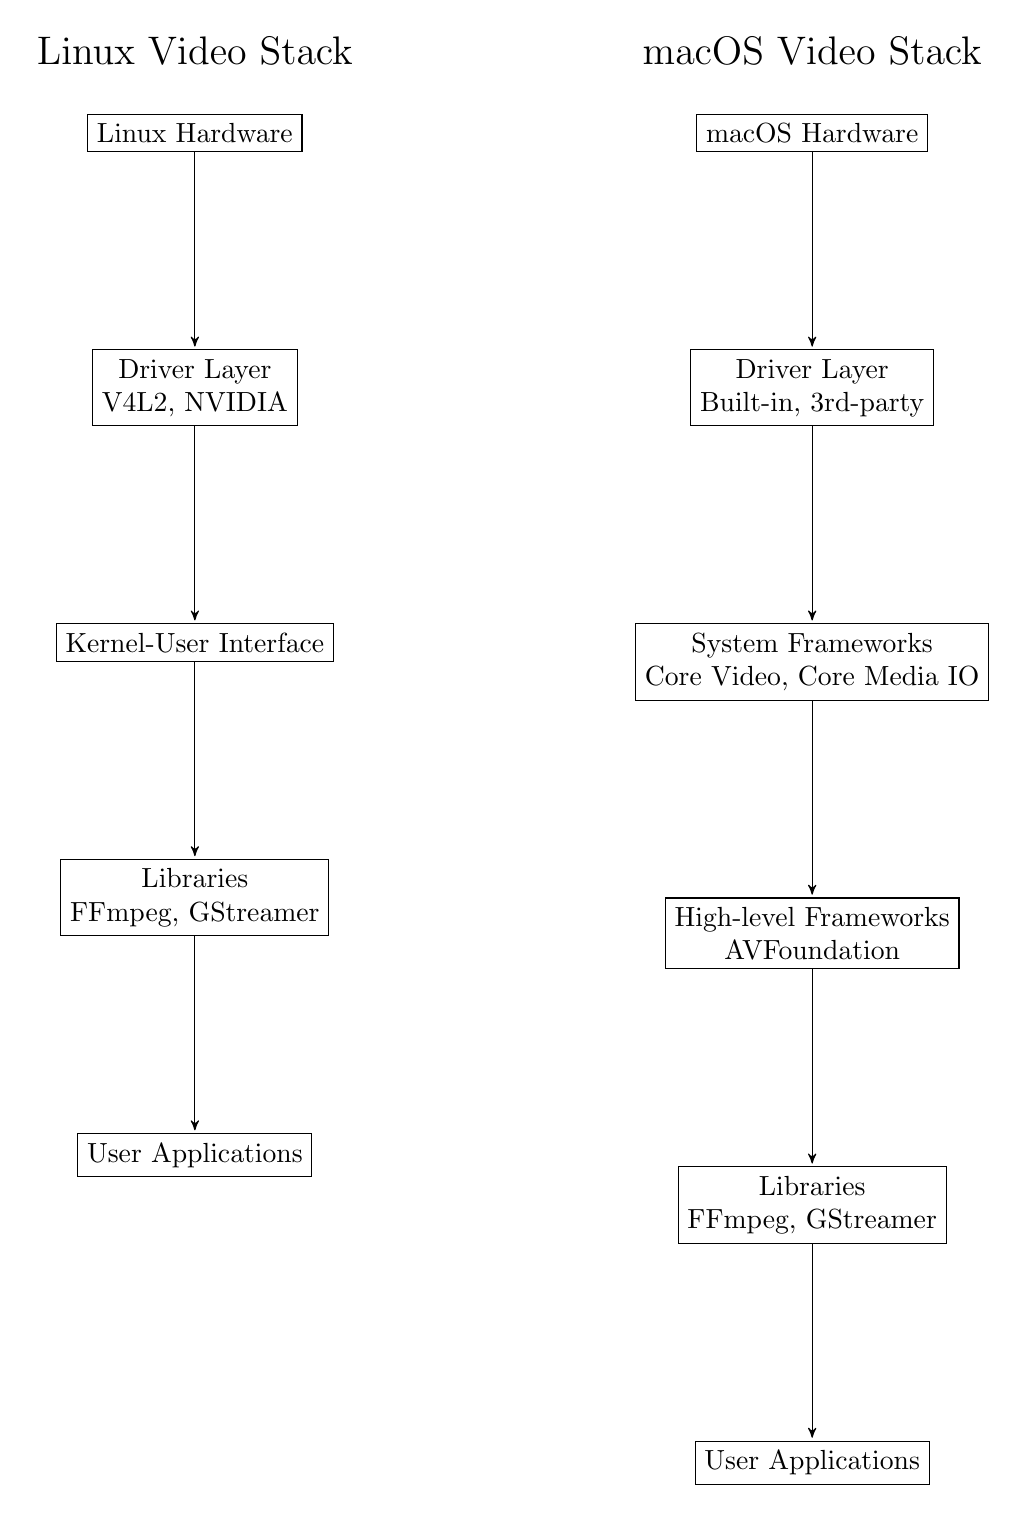
\begin{tikzpicture}[>=stealth', shorten >=1pt, auto, node distance=2.5cm]
    % Linux Stack
    \node (LinuxHardware) [draw, rectangle, align=center] {Linux Hardware};
    \node (LinuxDriver) [below=of LinuxHardware, draw, rectangle, align=center] {Driver Layer\\V4L2, NVIDIA};
    \node (LinuxKernelUser) [below=of LinuxDriver, draw, rectangle, align=center] {Kernel-User Interface};
    \node (LinuxLibraries) [below=of LinuxKernelUser, draw, rectangle, align=center] {Libraries\\FFmpeg, GStreamer};
    \node (LinuxApps) [below=of LinuxLibraries, draw, rectangle, align=center] {User Applications};
    
    % macOS Stack
    \node (MacHardware) [right=5cm of LinuxHardware, draw, rectangle, align=center] {macOS Hardware};
    \node (MacDriver) [below=of MacHardware, draw, rectangle, align=center] {Driver Layer\\Built-in, 3rd-party};
    \node (MacSysFrameworks) [below=of MacDriver, draw, rectangle, align=center] {System Frameworks\\Core Video, Core Media IO};
    \node (MacHighFrameworks) [below=of MacSysFrameworks, draw, rectangle, align=center] {High-level Frameworks\\AVFoundation};
    \node (MacLibraries) [below=of MacHighFrameworks, draw, rectangle, align=center] {Libraries\\FFmpeg, GStreamer};
    \node (MacApps) [below=of MacLibraries, draw, rectangle, align=center] {User Applications};
    
    % Arrows and Descriptions
    \draw[->] (LinuxHardware) -- (LinuxDriver);
    \draw[->] (LinuxDriver) -- (LinuxKernelUser);
    \draw[->] (LinuxKernelUser) -- (LinuxLibraries);
    \draw[->] (LinuxLibraries) -- (LinuxApps);
    
    \draw[->] (MacHardware) -- (MacDriver);
    \draw[->] (MacDriver) -- (MacSysFrameworks);
    \draw[->] (MacSysFrameworks) -- (MacHighFrameworks);
    \draw[->] (MacHighFrameworks) -- (MacLibraries);
    \draw[->] (MacLibraries) -- (MacApps);
    
    % Labels
    \node [above=0.5cm of LinuxHardware, font=\Large] {Linux Video Stack};
    \node [above=0.5cm of MacHardware, font=\Large] {macOS Video Stack};
    
\end{tikzpicture}

\end{document}

